
%(BEGIN_QUESTION)
% Copyright 2010, Tony R. Kuphaldt, released under the Creative Commons Attribution License (v 1.0)
% This means you may do almost anything with this work of mine, so long as you give me proper credit

Calculate all voltages, currents, and total power in this balanced three-phase system where a Delta-connected source provides electrical power to a 250 horsepower Y-connected motor.  Assume the motor operates at full load (100\% power) with perfect power factor and perfect efficiency:

$$\includegraphics[width=15.5cm]{i02448x01.eps}$$

\begin{itemize}
\item{} $E_{line} =$
\vskip 10pt
\item{} $I_{line} =$
\vskip 10pt
\item{} $E_{phase(source)} =$
\vskip 10pt
\item{} $I_{phase(source)} =$
\vskip 10pt
\item{} $E_{phase(load)} =$
\vskip 10pt
\item{} $I_{phase(load)} =$
\vskip 10pt
\item{} $P_{total} =$
\end{itemize}

\vskip 20pt \vbox{\hrule \hbox{\strut \vrule{} {\bf Suggestions for Socratic discussion} \vrule} \hrule}

\begin{itemize}
\item{} Identify which fundamental principles of electric circuits apply to each step of your analysis of this circuit.  In other words, be prepared to explain the reason(s) ``why'' for every step of your analysis, rather than merely describing those steps.
\item{} How might the results differ if the motor output the same amount of mechanical power, but at a lesser efficiency level (i.e. $<$ 100\%)?
\item{} How might the results differ if the power factor were less than 1?
\end{itemize}

\underbar{file i02448}
%(END_QUESTION)





%(BEGIN_ANSWER)

\noindent
{\bf Partial answer:}

\begin{itemize}
%\item{} $E_{line} =$ 4160 V
\item{} $I_{line} =$ 25.88 A
%\item{} $E_{phase(source)} =$ 4160 V
\item{} $I_{phase(source)} =$ 14.94 A
\item{} $E_{phase(load)} =$ 2402 V
%\item{} $I_{phase(load)} =$ 25.88 A
%\item{} $P_{total} =$ 186.5 kW
\end{itemize}

%(END_ANSWER)





%(BEGIN_NOTES)

\begin{itemize}
\item{} $E_{line} =$ 4160 V
\item{} $I_{line} =$ 25.88 A
\item{} $E_{phase(source)} =$ 4160 V
\item{} $I_{phase(source)} =$ 14.94 A
\item{} $E_{phase(load)} =$ 2402 V
\item{} $I_{phase(load)} =$ 25.88 A
\item{} $P_{total} =$ 186.5 kW
\end{itemize}

\vskip 10pt

Be sure to ask your students to describe {\it how} they arrived at the answers to this question.  There is more than one place to start in determining the solution here, and more than one way to calculate some of the figures.  No matter how your students may have approached this question, though, they should all obtain the same answers.

%INDEX% Electronics review: 3-phase voltage/current/power calculation

%(END_NOTES)



